\documentclass[11pt, a4paper]{article}
\usepackage[utf8]{inputenc}
\usepackage[slovene]{babel}
\usepackage{amsmath}
\usepackage{graphicx}
\usepackage{hyperref}

\title{Domača naloga: Naravni kubični zlepek}
\author{Anže Judež}
\date{\today}

\begin{document}

\maketitle

\section{Splošen opis naloge}
Cilj naloge je bila implementacija naravnega kubičnega zlepka $S(x)$ za dano množico interpolacijskih točk $(x_i, f_i)$ za $i = 1, \dots, n$ \cite{textbook}. Po navodilih mora funkcija izpolnjevati naslednje pogoje \cite{textbook}:
\begin{itemize}
    \item $S(x_i) = f_i$ za vse $i = 1, \dots, n$.
    \item $S$ je polinom stopnje 3 ali manj na vsakem podintervalu $[x_i, x_{i+1}]$.
    \item $S$ je dvakrat zvezno odvedljiva funkcija na celotnem intervalu.
    \item Naravna robna pogoja sta $S''(x_1) = S''(x_n) = 0$.
\end{itemize}

\section{Splošen opis rešitve}
Zlepek določimo tako, da na vsakem podintervalu $[x_i, x_{i+1}]$ postavimo polinom \cite{textbook}:
\[ S_i(x) = a_i + b_i(x - x_i) + c_i(x - x_i)^2 + d_i(x - x_i)^3 \]

Reševanje sistema enačb smo prilagodili strukturi problema. Namesto uporabe splošnih metod smo izkoristili dejstvo, da določanje parametrov vodi do tridiagonalne matrike \cite{textbook}. S tem smo časovno zahtevnost algoritma zmanjšali na zgolj $O(n)$ \cite{textbook}. V poročilu se izogibamo podrobni razlagi kode in se raje osredotočamo na matematični opis postopka, kjer koeficiente $c_i$ dobimo z reševanjem sistema, preostale parametre pa izpeljemo iz pogojev za zveznost \cite{textbook}.

\section{Primer uporabe}
Za testiranje algoritma smo uporabili vzorčne podatke. Na sliki \ref{fig:zlepek} je prikazan izračunan naravni kubični zlepek. Različni barvni odseki ponazarjajo posamezne polinome $S_i$, ki se v stičiščih gladko povezujejo, kar potrjuje zveznost odvodov \cite{textbook}.

\begin{figure}[h]
    \centering
    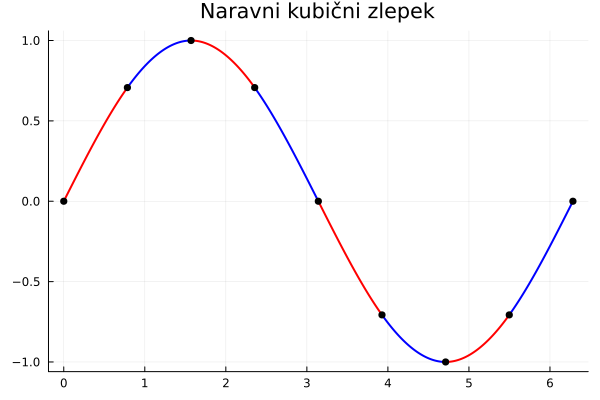
\includegraphics[width=0.8\textwidth]{zlepek_sinus.png}
    \caption{Graf naravnega kubičnega zlepka.}
    \label{fig:zlepek}
\end{figure}

\section{Navodila za uporabo}
Koda je pripravljena v programskem jeziku Julia in organizirana kot paket \texttt{Naloga01} \cite{textbook}.
\begin{itemize}
    \item \textbf{Zagon testov:} V Julia REPL vpišite \texttt{using Pkg; Pkg.test("Naloga01")}.
    \item \textbf{Izračun:} Uporabite funkcijo \texttt{interpoliraj(x, y)}, ki vrne tip \texttt{Zlepek}.
    \item \textbf{Poročilo:} Za generiranje grafov za poročilo zaženite skripto \texttt{demo.jl}.
\end{itemize}

\begin{thebibliography}{9}
\bibitem{textbook} 
M. Vuk, \textit{Navodila za pripravo domačih nalog in opisi nalog (poglavja 17 in 18)}, Učbenik za numerične metode, 2026.
\end{thebibliography}

\end{document}